\documentclass[12pt,a4paper]{article}
\usepackage[utf8]{inputenc}
\usepackage{amsmath}
\usepackage{amsfonts}
\usepackage{amssymb}
\usepackage{lmodern}
\usepackage[toc]{appendix}
\usepackage{graphicx}
\renewcommand{\baselinestretch}{1}
\usepackage[final]{pdfpages}



%Header packages
\usepackage{fancyhdr}
 %%%%%%%%%%%%%%%%%%%%%%%%%%%%55
 %Might change header back later
\pagestyle{fancy}
\fancyhf{}
\rhead{MAY1607}
\lhead{Microscope HUD}
\rfoot{Page \thepage}




%\author{Noah Bergman}
%\title{Heads-Up Display for a Manufacturing Microscope}




\usepackage{tikz}
\usepackage{epigraph}
\usepackage{lipsum}

\renewcommand\epigraphflush{flushright}
\renewcommand\epigraphsize{\normalsize}
\setlength\epigraphwidth{0.7\textwidth}

\definecolor{titlepagecolor}{cmyk}{1,.60,0,.40}

\DeclareFixedFont{\titlefont}{T1}{ppl}{b}{}{0.5in}

\makeatletter                       
\def\printauthor{%                  
    {\large \@author}}              
\makeatother
\author{%
    \textbf{Prepared By:} \\
    	\begin{flushright}
    		Noah Bergman,\\
    		Greg Kuhn, \\
    		Mike Kelly, \\
    		Garrett Hembry
    	\end{flushright}
%    Department name \\
%    \texttt{email1@example.com}\vspace{20pt} \\
%    Author 2 name \\
 %   Department name \\
%    \texttt{email2@example.com}
    }

% The following code is borrowed from: http://tex.stackexchange.com/a/86310/10898

\newcommand\titlepagedecoration{%
\begin{tikzpicture}[remember picture,overlay,shorten >= -10pt]

\coordinate (aux1) at ([yshift=-15pt]current page.north east);
\coordinate (aux2) at ([yshift=-410pt]current page.north east);
\coordinate (aux3) at ([xshift=-4.5cm]current page.north east);
\coordinate (aux4) at ([yshift=-150pt]current page.north east);

\begin{scope}[titlepagecolor!40,line width=12pt,rounded corners=12pt]
\draw
  (aux1) -- coordinate (a)
  ++(225:5) --
  ++(-45:5.1) coordinate (b);
\draw[shorten <= -10pt]
  (aux3) --
  (a) --
  (aux1);
\draw[opacity=0.6,titlepagecolor,shorten <= -10pt]
  (b) --
  ++(225:2.2) --
  ++(-45:2.2);
\end{scope}
\draw[titlepagecolor,line width=8pt,rounded corners=8pt,shorten <= -10pt]
  (aux4) --
  ++(225:0.8) --
  ++(-45:0.8);
\begin{scope}[titlepagecolor!70,line width=6pt,rounded corners=8pt]
\draw[shorten <= -10pt]
  (aux2) --
  ++(225:3) coordinate[pos=0.45] (c) --
  ++(-45:3.1);
\draw
  (aux2) --
  (c) --
  ++(135:2.5) --
  ++(45:2.5) --
  ++(-45:2.5) coordinate[pos=0.3] (d);   
\draw 
  (d) -- +(45:1);
\end{scope}
\end{tikzpicture}%
}





\begin{document}
%\maketitle
\begin{titlepage}

\noindent
\titlefont Heads-Up Display for a Manufacturing Microscope\par
%\epigraph{Pure mathematics is on the whole distinctly more useful than applied. For what is useful above all is technique, and mathematical technique is taught mainly through pure mathematics.}%
%{\textit{London 1941}\\ \textsc{G. H. Hardy}}
\null
\vspace*{1cm}
\noindent
\begin{minipage}{0.5\textwidth}
    \begin{flushleft}
    \printauthor
    \end{flushleft}
\end{minipage}
%\begin{minipage}{0.1\textwidth}
	%\rule{1pt}{pt}
%\end{minipage}
\vspace{1in}
\\
\begin{minipage}{0.5\textwidth}
    \begin{flushleft}
    \large
    \textbf{Submitted To:}
    	\begin{flushright}
    		\textbf{Bob Dearth}\\
    		Honeywell Intl. Inc. \\
    		~\\
    		\textbf{Dr. Jaeyoun Kim }\\
    		Iowa State University\\
    		~\\
    		\textbf{Dr. George Amariucai}\\
    		Iowa State University
   		\end{flushright}
    \end{flushleft}
\end{minipage}
%
\titlepagedecoration
\end{titlepage}
\pagebreak

%%%%%%%%%%%%%%%%%%%%%%%%%%%%%%%%%%%%%%%%%%%%%%%%%%%%%%%%%%%%%%%%%%%%%%%%%%%5

\tableofcontents

\listoffigures

%\listoftables

\pagebreak
%%%%%%%%%%%%%%%%%%%%%%%%%%%%%%%%%%%%%%%%%%%%%%%%%%%%%%%%%%%%%%%%%%%%%%%%%%%%%%%%%
\section{Introduction}
Honeywell technicians assemble miniature mechanisms under a microscope. They face repetitive movements and eye strain while checking work instructions which are displayed on a nearby computer. A Kansas State design team outlined several solutions to this problem: a small tablet mounted next to the microscope, a virtual environment using technology similar to the Oculus Rift, and a heads up display inside the microscope’s field of view. We are exploring the last of these options. 



%%%%%%%%%%%%%%%%%%%%%%%%%%%%%%%%%%%%%%%%%%%%%%%%%%%%%%%%%%%%%%%%%%%%%%%%%%%%%%
\section{Project Statement}
Optically inserting a virtual screen inside the microscope’s field of view allows the operator to seamlessly refer to work instructions during assembly. This setup could potentially improve workplace ergonomics and reduce manufacturing time while ensuring all components meet Honeywell’s high quality expectations. 

\section{Design Requirements}

\begin{itemize}
	\item Allows users to interact with PDFs that contain embedded pictures, videos, and links to other work instructions.
	\item Does not obstruct the 15” vertical workspace below the objective lens.
	\item Does not restrict airflow in the workspace to maintain ISO Class 7 clean room standards.
	\item Remains in focus during normal microscope operation.
\end{itemize}

\section{Deliverables}
\begin{itemize}
	\item Design workking prototype of heads-up display system.
	\item Provide all design documents, schematics, and code.
	\item Operations Manual to demonstrate how to setup and use the system.
	\item Future design manual that outlines improvements and ideas for development down the line.
\end{itemize}


%%%%%%%%%%%%%%%%%%%%%%%%%%%%%%%%%%%%%%%%%%%%%%%%%%%%%%%%%
\section{Functional Overview}
To meet all the requirements, our group designed a DLP projector with custom optics, hardware, and firmware. Our design is centered around the Texas Instruments’ DLP3010 chipset and uses the DLP3010 EVM optical engine and DLP controller board.  The entire system can be broken down into three main parts: main control board, DLP control board, and the optical system. These subsystems work together to display the final image inside the microscope. Figure \ref{block_diagram} shows the block diagram of the final design.

\begin{figure}[h!]
	\centering
	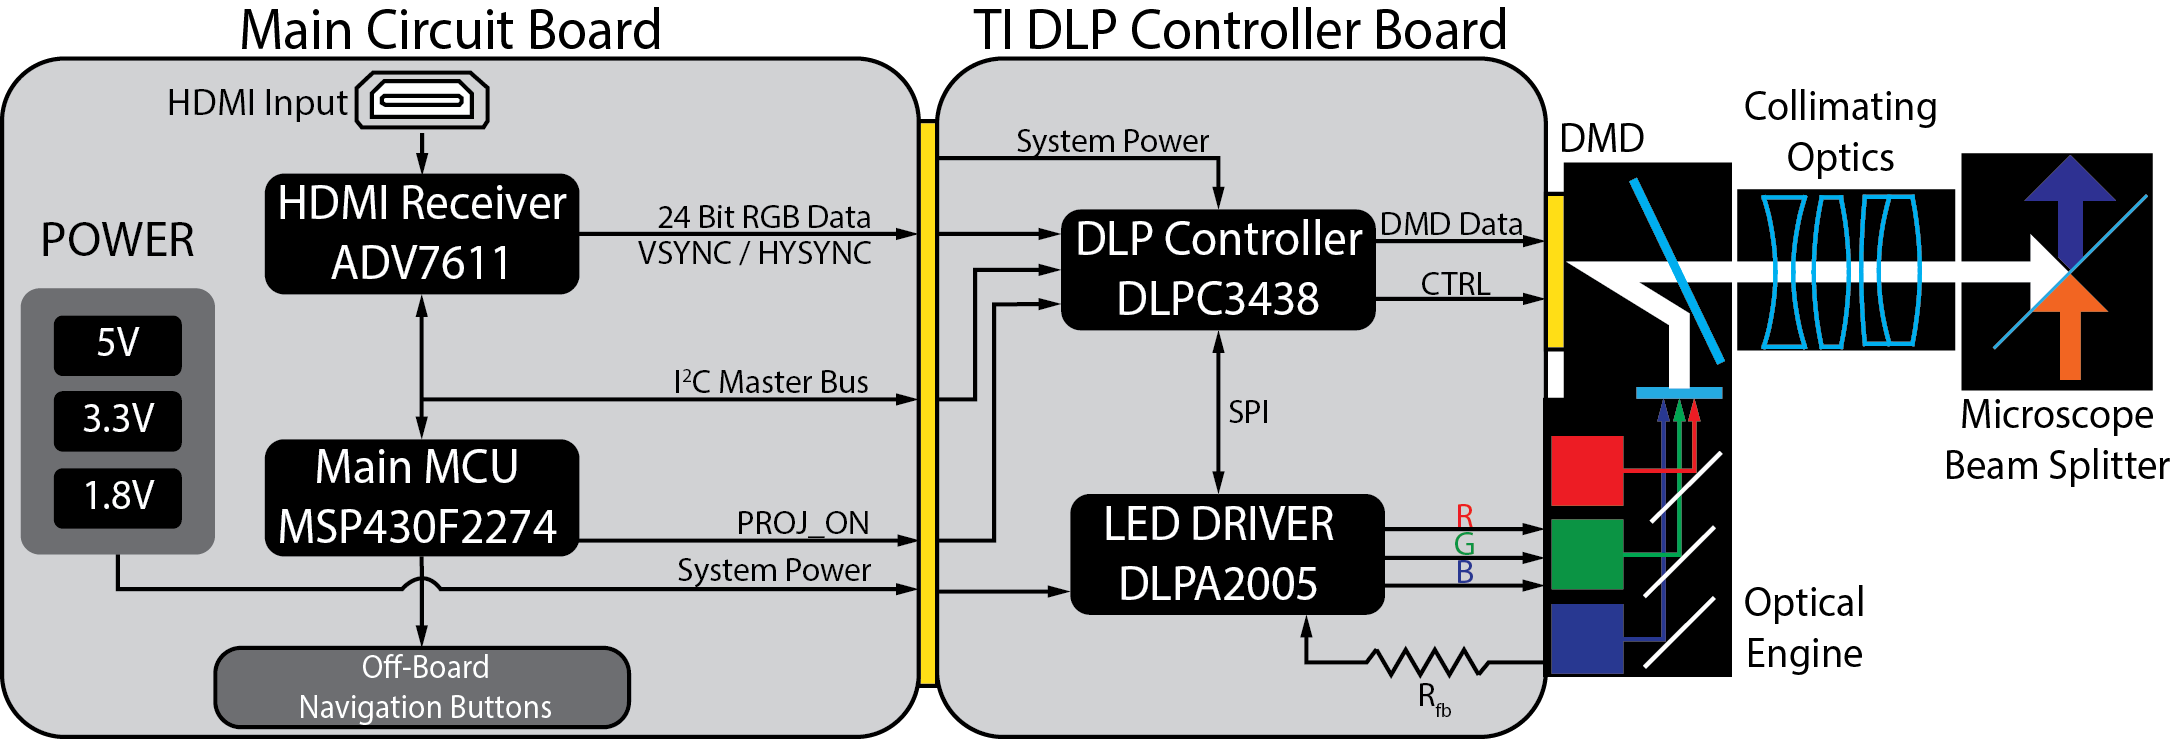
\includegraphics[width = \textwidth]{pics/seniorDesign_blockDiagram.png}
	\caption[Block Diagram]{Block diagram of the main board, DLP controller, and Optical system}
	\label{block_diagram}
\end{figure}


\subsection{Main Control Board}
The main control board was designed to take an HDMI input and convert the data to 24 bit RGB format which is fed directly to the DLP3438 display controller. The on-board microcontroller, MSP430F2274, serves as both a user interface hub and system coordinator. The power-on switch and navigation buttons are connected GPIOs. These inputs are configured in software to trigger certain events in the projector. For example, the left and right buttons can be used to change screen size, zoom, and cropping while the power switch simply triggers all the initialization code to run. The MCU communicates with both the ADV7611 and the DLPC3438 over I\textsuperscript{2}C. All the power for the system is routed through the main board. The 5V input is stepped down to 3.3V and 1.8V using buck regulators. 

\subsection{DLP Controller}
The DLP controller board was part of an evaluation kit from Texas Instruments. The board consists of the DLPC3438 display controller and the DLPA2005 PMIC / LED driver. These two integrated circuits work in tandem to control the DLP3010, digital micro-mirror device.

\subsection{Optical System}
This optical engine uses three LEDs, red, green, and blue, to project a full color image. The light is combined and reflected off the DMD and out through the custom optical system. The optics we designed take the projected light, magnify, correct for aberrations, and finally collimate the image before it is sent into the infinity space of the microscope. The EMZ-8TRU has a camera port attachment that was removed and modified to change the direction of the beam splitter. This allowed the image to be reflected up through the eyepiece where the user can view the virtual screen.




%%%%%%%%%%%%%%%%%%%%%%%%%%%%%%%%%%%%%%%%%%%%%%%%%%%%%%%%%%%%%%%
\section{Detailed Hardware Design}

\subsection{Main Control Board}
\subsubsection{HDMI Receiver - ADV7611}
The ADV7611 receives HDMI signals from the input source, converts the data format, and provides display information to the source over I\textsuperscript{2}C. Before any pixel data can be transferred, the source must know some basic information about the display. The External Device ID is 128 bytes of data that holds manufacturer information, serial number, display dimensions, data speeds, and color information. The final byte holds a check-sum of the data block. Once this information has been transferred over and a confirmation has been sent, both devices are ready to communicate.

The image data is transmitted over four differential pair wires, three for data and one for clock, at 60 frames per second for 1080p displays. This corresponds to a data rate of 3.4Gbps. Routing high speed signals on a circuit board requires special attention. The propagation delay of the signal is directly proportional to the dielectric of fiberglass and length of trace. This becomes incredibly crucial for differential pairs as a mismatch in timing can cause excess power draw on the lines or even corrupt data. 

The ADV7611 converts the video into 24 bit RGB format. This parallel interface uses 8 bits per color per pixel. Each pixel is clocked in like a typewriter, each pixel placed to the right of the previous. At the end of each line, the HSYNC line is pulsed, notifying the receiver to start the next line. The last row of pixels is clocked in and followed by a pulse on the VSYNC line. The receiver sets up for the next frame in the same manner as before, starting in the corner and clocking across.



\subsubsection{Microcontroller - MSP430F2274}
The on-board MSP430F2274 acts as the main coordinator for the system. The DLP controller and ADV7611 are both controlled via I\textsuperscript{2}C. All settings and events are routed through the microcontroller and sent to the respective chip. 
%%%% Add schematic

\subsubsection{Power}
Finally, the main board acts as the power distribution center. The 5V system power is converted to 1.8V and 3.3V using two switching regulators. All three control voltages are necessary for normal operation. When power is first applied, the system waits for the 5V and 3.3V power to stabilize before turning on the 1.8V supply. This power-up sequence is necessary for a clean program start and ensures none of the components are damaged. 
%%% Add schematic
\begin{figure}[h!]
	\centering
	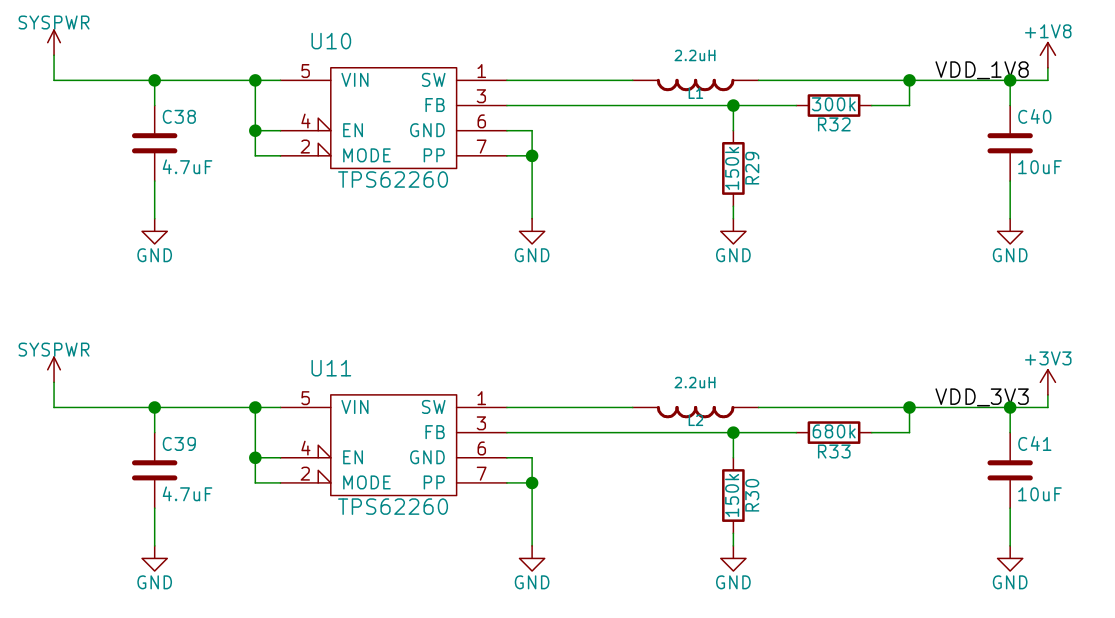
\includegraphics[width = \textwidth]{pics/powerReg.png}
	\caption[Power Regulator Schematic]{\centering The 3.3V and 1.8V voltage regulator circuit.}
\end{figure}

%%%%%%%%%%%%%%%%%%%%%%%%%%%%%%%%%%%%%%%%%%%%5
\subsection{DLP Controller Board}

\subsubsection{DMD Controller - DLPC3438}
The DLPC3438 directly controls the DMD and the LED driver. The control chip only takes in 24 bit RGB data, but can also render its own splash screens and test patterns. The MSP430 can call specific operations over I\textsuperscript{2}C such as, image cropping, changing brightness, image angle, and many more. 

\subsubsection{LED Controller - DLPA2005}
The DLPA2005 uses a feedback resistor on the cathode side of the LEDs to track current. An internal DAC is set to limit LED current, the output is compared to the voltage across the shunt resistor and the channel is pulsed off until the current comes back within range. The original value of 39m$\Omega$ was intended for current control between 1.5 and 2.1 amps per channel. This device was originally designed to produce 150 lumens and was not intended for direct line of sight out of the box. Replacing the original with a 100$\Omega$ resistor allowed us to test the LEDs down to a few milliamps. 

\subsection{Optical Design}
\subsubsection{Modified Optical Engine}
Projector optical engines are not designed to work while facing the display. Removing the projection optics reveals the small DMD hidden inside. The small rectangle glows brilliantly as the thousands of tiny mirrors silently toggle back and forth. DLP systems typically use a white bulb with a color wheel or colored LEDs to generate the full color spectrum. 

\subsubsection{Collimating Optics}
The lens system was designed to collimate the image projected directly from the DMD. Our system uses three different types of lens to tweak various aspects of our system.
\paragraph{Bi-Concave}
	The Bi-Convex lens has a focal length of -30mm and is placed approximately 34.5mm away from the DMD. This produces a smaller virtual image within range of the second lens.
\paragraph{Bi-Convex}
This intermediate lens magnifies the virtual image and prepares it for the final collimation. This lens makes it easy to fine tune the balance between longer focal length and apparent image size.
\paragraph{Achromatic Bi-Convex}
The final lens consists of two different materials glued together. The difference in the index of refractions corrects for color aberrations in the image. The final image is much clearer because the colors all collimate together.

\begin{figure}[h!]
	\centering	
	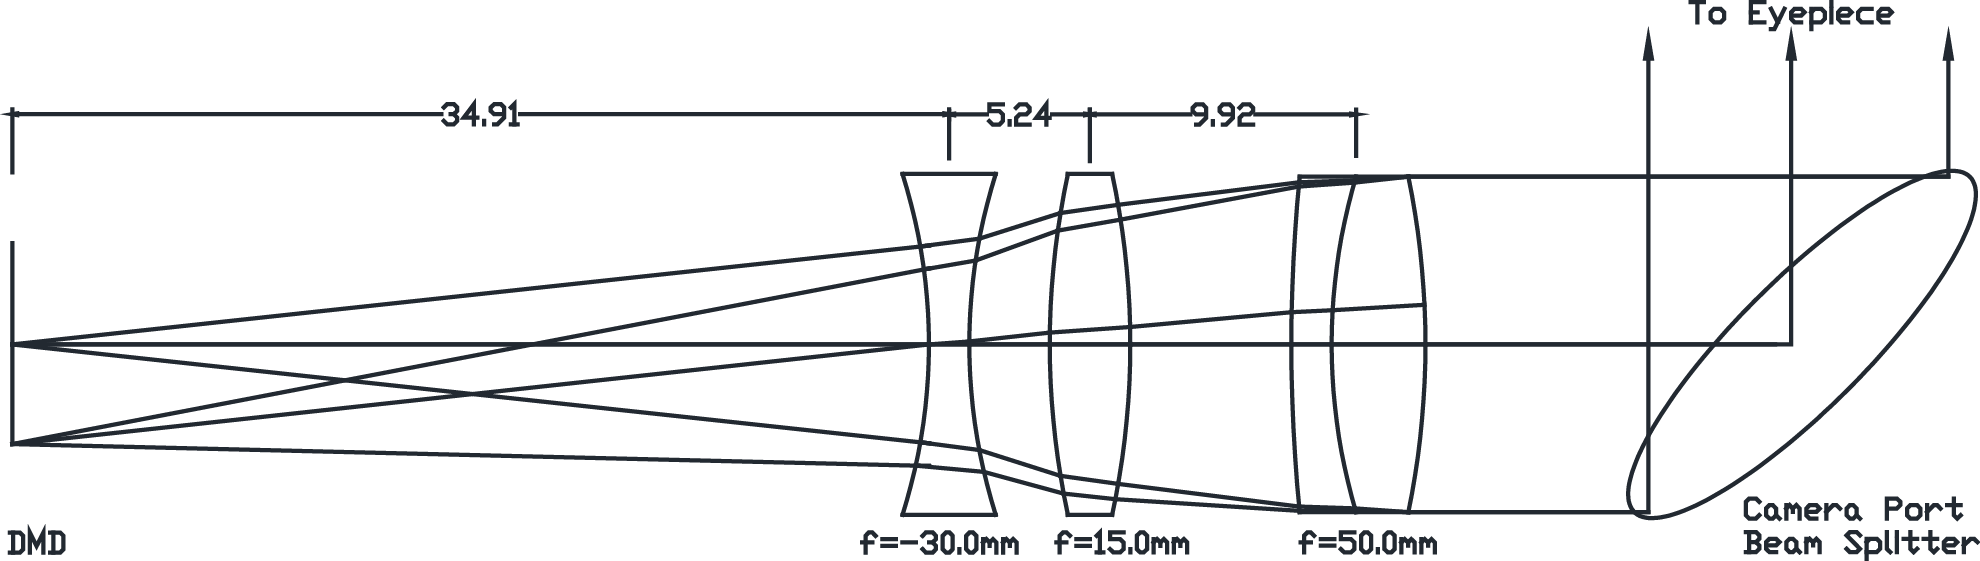
\includegraphics[width = \textwidth]{pics/LENSdRAWING.png}
	\caption[Optics Diagram]{The optical schematic}
\end{figure}

\section{Testing}
\subsection{Objective Lens Integration}
When this project began, testing consisted purely of attempting to send any sort of light through the microscope and receiving it at the eyepieces. The simplest method to test this was to implement the projector circuit below the objective lens. After this initial proof of concept was developed, the complexity of testing increased. The next task was to prove it was possible to project an image through the microscope for the user to see. The beam splitter is placed at a specific angle below the objective lens, and the projector was able to reflect an image up into the objective lens for the user to see. Unfortunately, the light received from the projector was much too bright. In order to dim the light from the LED, more resistance was added to the projector circuit.

After the brightness issue was resolved, it became apparent that much of the available workspace below the microscope was now being occupied by our setup under the microscope. To decrease the amount of workspace used by our project, we modified the angle between the beam splitter and the objective lens. To free up the workspace for the lab technicians we made incremental adjustments until we found the smallest working angle that still provided an acceptable quality image to the user. The image received had its own issues as well, so alternative ways to implement the system to improve the image quality were sought out. 

\subsection{Camera Port Integration}
Implementing the setup in the camera port relocated our circuitry so that it was completely out of the workspace and also allowed for the use of more precise optics that were already in place. With some slight modifications to these optics the image could be projected through the microscope to the eyepiece with little outside interaction. The resulting image was much clearer and legible. The next step was to use actual work instructions as the projected image to determine the legibility of text instructions. After this step in testing, it was determined that the text instructions could successfully be projected through the microscope and read by the microscope operator using our setup. 

Much of the remaining testing process for this concept dealt with the creation of custom hardware in order to hold and house our projector circuit in the most optimal way. The first iteration of this hardware simply attached our optical system to the microscope, and we quickly realized the hardware would also need to hold and support the rest of the circuit in addition to attaching the system to the microscope. The final version of the hardware would not only house the circuit and attach it to the microscope, but it would also allow for the optical system to be adjusted when necessary.

\section{Conclusion}

During these past two semesters of senior design we managed to successfully create a heads-up display and integrate it into a microscope. In order to get this product working successfully we
used many skills from varying branches of science and engineering. We had to employ our knowledge of optics and lenses, 3D-modeling, circuit design, and microcontrollers to create a working heads up display. Overall, this was a fascinating and worthwhile project where we managed to successfully complete our project using creative problem solving and teamwork.



\pagebreak
%Begin the appendix
\begin{appendices}

\section{Operation Manual}

\begin{enumerate}
	\item Prepare the Workspace
	\begin{itemize}
		\item Set up the microscope by attaching the stand and the microscope together.
	\end{itemize}
	\item Modify the Existing System
	\begin{itemize}
		\item Remove the camera port and replace with a modified version.
		\begin{itemize}
			\item Attach the unit securely, as it will hold the lenses which are sensitive to small changes in alignment.
		\end{itemize}
	\end{itemize}
	
	\item Optical Setup
		\begin{itemize}
			\item The lens configuration should be placed in the lens tube.
			\begin{itemize}
				\item Place lens at the focal point to ensure optimal image quality.
			\end{itemize}
			\item Insert the lens tube securely into thelens housing apparatus.
		\end{itemize}
	
	\item Circuit Setup
		\begin{itemize}
			\item Attach the projector circuit to the modified camera port
			\item Power the circuitry via and electrical outlet
			\item Connect the projector to the storage system containing instruction document
			\item Activate the projector by turning on the switch
		\end{itemize}
	
	\item User Information
		\begin{itemize}
		
			\item The image will be displayed into the eyepiece of the microscope
			\item Toggle between the workspace view and the instructions by powering on and off the system
		\end{itemize}
\end{enumerate}

\section{Alternative Designs}
\subsection{Objective Lens Integration}
Our design process began by brainstorming various methods of inserting a projection into the microscope system.  With our intentions focused only on providing the instructions directly to the user, we predicted three potential points of insertion.  These projection possibilities ranged from the area immediately in contact with the user (the eyepiece), to a portion of the optics tangential to the overall system (the camera port), and also the portion of the microscope already being used to capture images (the objective lens).

We decided to pursue a strategy that utilized the objective lens as the insertion point of the projected image for our first design.  This was a result of the compactness of the eyepiece component, which had no tolerance for customization, and also that the default position of the camera port system allowed only for image capture.  Later it became apparent that the camera port could be changed to display an image to the eyepiece, which we took advantage of at a point farther along in the design process.
	
Because the objective lens’ purpose is to capture light and display it to the user, pursuing this design allowed us to focus more on the projection system as a first priority.  We began by purchasing a commercial projector for testing of the various lens and component setups to be used in conjunction with an image source.  This was chosen as a way of getting immediate feedback on the methods of focusing the image as it traveled to the objective lens.  It is relevant to note that as a result of our project being almost completely hardware oriented, progressing through suggested concepts requires actual testing, and so many of our designs are focused on allowing us to get results on feasibility and quality in a very short time frame.

As part of experimenting with the various lens arrangements and several different beam splitters, it was necessary to disassemble and adapt the purchased pocket projector to better fit our needs.  We removed all of the casing and added a small circuit board attachment to optimize the brightness setting of the projector.  We were then able to find the correct beam splitter alignment in conjunction with the projector’s position so that the image would be viewed properly in the eyepiece.  This was very important because as the light travels through the microscope system, the image is reflected off of many surfaces and is displayed in a different orientation than was initially projected at the beginning of the process.

The final part of our design required us to build a physical structure to not only hold each of the components in their particular positions, but also to attach them securely to the microscope itself.  The resulting model is shown in Figure \ref{OLS}, where the beam splitter is placed just below the objective lens with the projector and its controlling circuitry held to the side.  The projector and beam splitter are placed at specific angles so that the image is reflected directly into the objective lens, but while the power is off, the beam splitter allows for the view below the system to enter into the lens unobstructed.

\begin{figure}[h]
	\centering
	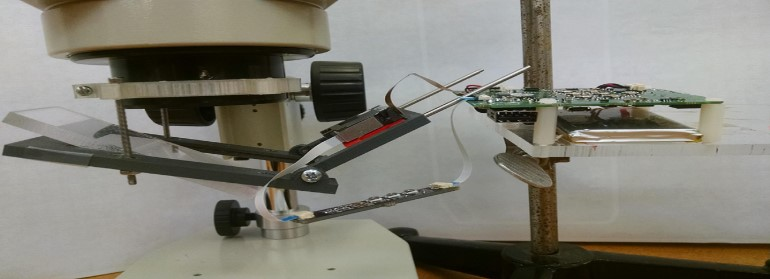
\includegraphics[width = 0.75\textwidth]{pics/objective_lens_setup.jpg}
	\caption[Objective Lens Setup]{\centering Design using modified commercial projector underneath the objective lens.}
	\label{OLS}
\end{figure}


This was a good result for our first design, but there were several disadvantages that we wanted to optimize as our project developed.  The main issue with the objective lens integration setup was that the angle of reflection required the beam splitter and projector to be placed in the user’s workspace.  We built our model in such a way so that the components were held off to the side, but this design still posed a considerable obstruction to the workstation.  Another topic of concern was that the distance between the projector and beam splitter needed to be adjusted each time the zoom of the microscope was changed.  This is because the focal point of the projection system needed to be changed in accordance to the magnification being viewed by the user.  Finally, the projected image presented a double image when viewed (shown in Figure \ref{OLO}), which was a result of the beam splitter having two reflective surfaces.

\begin{figure}[h]
	\centering
	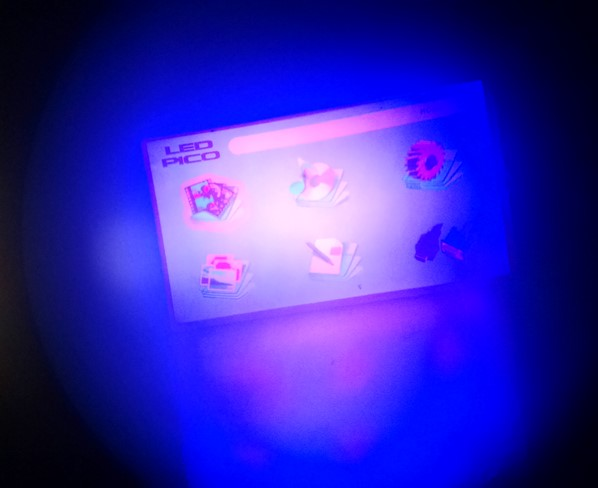
\includegraphics[width = 0.75\textwidth]{pics/objective_lens_output.jpg}
	\caption[Objective Lens Output]{\centering Image produced by the objective lens design as seen through eyepiece.}
	\label{OLO}
\end{figure}





\subsection{Camera Port Attachment}
As the project progressed, we were able to spend more time learning about the internal optics used in the microscope and to get more comfortable adjusting various parts of the system.  At one point we experimented with manipulating the set of mirrors used by the camera port in such a way so that they reflected light in a direction of our choosing.  This allowed us to change that part of the microscope which was only initially used for capturing images so that it could actually input a light source to be viewed by an eyepiece.

Once this development was made, we decided to pursue it as our second method of design for the project.  At this point we determined all of the necessary changes to be implemented for the new system.  This list included adjusting the camera port mirrors so that the image could be sent in a direction of our choosing, redesigning the camera port hardware itself to allow for easier input of images as well as to hold the project and other components being used.  We also knew that we would be able to change our beam splitter implementation completely, swapping in a lens array for focusing because we only needed to consider inserting the image as the camera port attachment does not obstruct the central optics used by the microscope.

In order to enact these changes we employed a few programs in conjunction with the usual testing and experimenting that is the staple of this project.  One program which was vital to determining the optimal distances used for the lens array that focused our image was WinLens 3D.  This optical simulation program not only allowed us to find those distances to be used, but also to test the impact that various types of lenses and optical components had on our projected image.  As shown in Figure \ref{LAD}, we went with a three lens system after completing the testing process with that program.  We utilized one biconcave and two biconvex lenses with achromatic lenses to correct for color aberration.

%WinLens -- TODO: Change to better stuff
\begin{figure}[h]
	\centering
	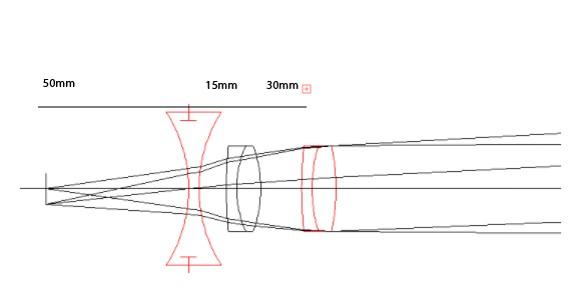
\includegraphics[width = 0.75\textwidth]{pics/lens_array.jpg}
	\caption[Lens Array Diagram]{\centering Lens array schematic with dimensions optimized by WinLens 3D software.}
	\label{LAD}
\end{figure}

Another useful software tool was the 3D modeling program, Solidworks, which was used to design two vital components for this optical integration method, shown in Figures \ref{LHM} and \ref{CPM}.  The first part that we needed to construct was a custom mounting bracket which would attach to the camera port and hold the focusing lenses in perfect alignment.  The second component that we needed to build became apparent after a few iterations of testing with the stock camera port, which had enough hindrances in its design that we eventually decided to construct our own version.  This was made so that we could integrate smoothly into the microscope with our projector and lens array, and also to provide support for our circuit board assembly.  After some testing with these new components, we came up with a few changes to the initial design and made a second model with optimized dimensions.


\begin{figure}[h!]
	\centering
	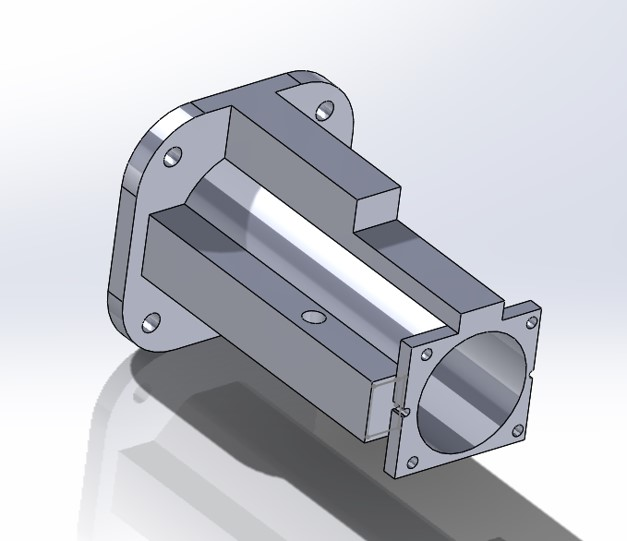
\includegraphics[width = 0.49\textwidth]{pics/lens_housing.jpg}
	\caption[Lens Housing Model]{\centering Custom lens mounting bracket to support the lenses used for focusing the image.}
	\label{LHM}
\end{figure}
\vfill
\begin{figure}[h!]
	\centering
	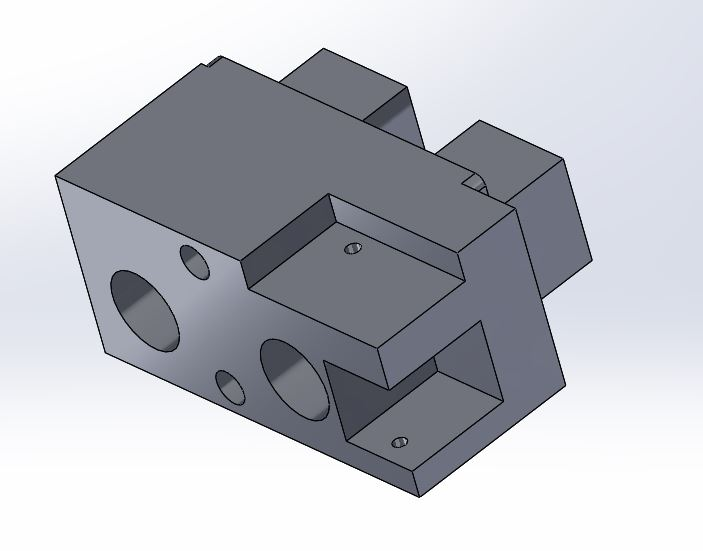
\includegraphics[width = 0.49\textwidth]{pics/camera_port.jpg}
	\caption[Camera Port Model]{\centering Custom camera port design to support the projector and house the lens array}
	\label{CPM}
\end{figure}

While we conducted tests for the physical parts just constructed, we also worked with the projection system to provide the best image through the optics housed in that hardware.  We made a small structural piece for the projector to provide support and attachment holes to lock it in place so that it remains aligned to the camera port. It was also necessary to design a custom PCB to remove all the unnecessary components not being used by the projector, which also helped to reduce the size and allow for easier integration on the camera port.  Part of this new PCB was a simple on/off switch which serves as the main control for our projection system and allows for easily displayed instructions once the system is attached.

There are several benefits that this new design has over our initial concept, the first of which concerns the focus of the displayed image.  Previously, any time the operator adjusted the magnification of his view he would then have to refocus our image before being able to view his instructions.  With this new design, our projection enters into the eyepiece directly from the camera port, meaning it is independent to the focus of the microscope system. Another advantage of our second concept is that all of our circuitry and optics are housed internally or held behind the microscope.  This keeps our attachment out of the workspace and enables for a much lower impact to the rest of the microscope system.


\section{Schemtic Files}
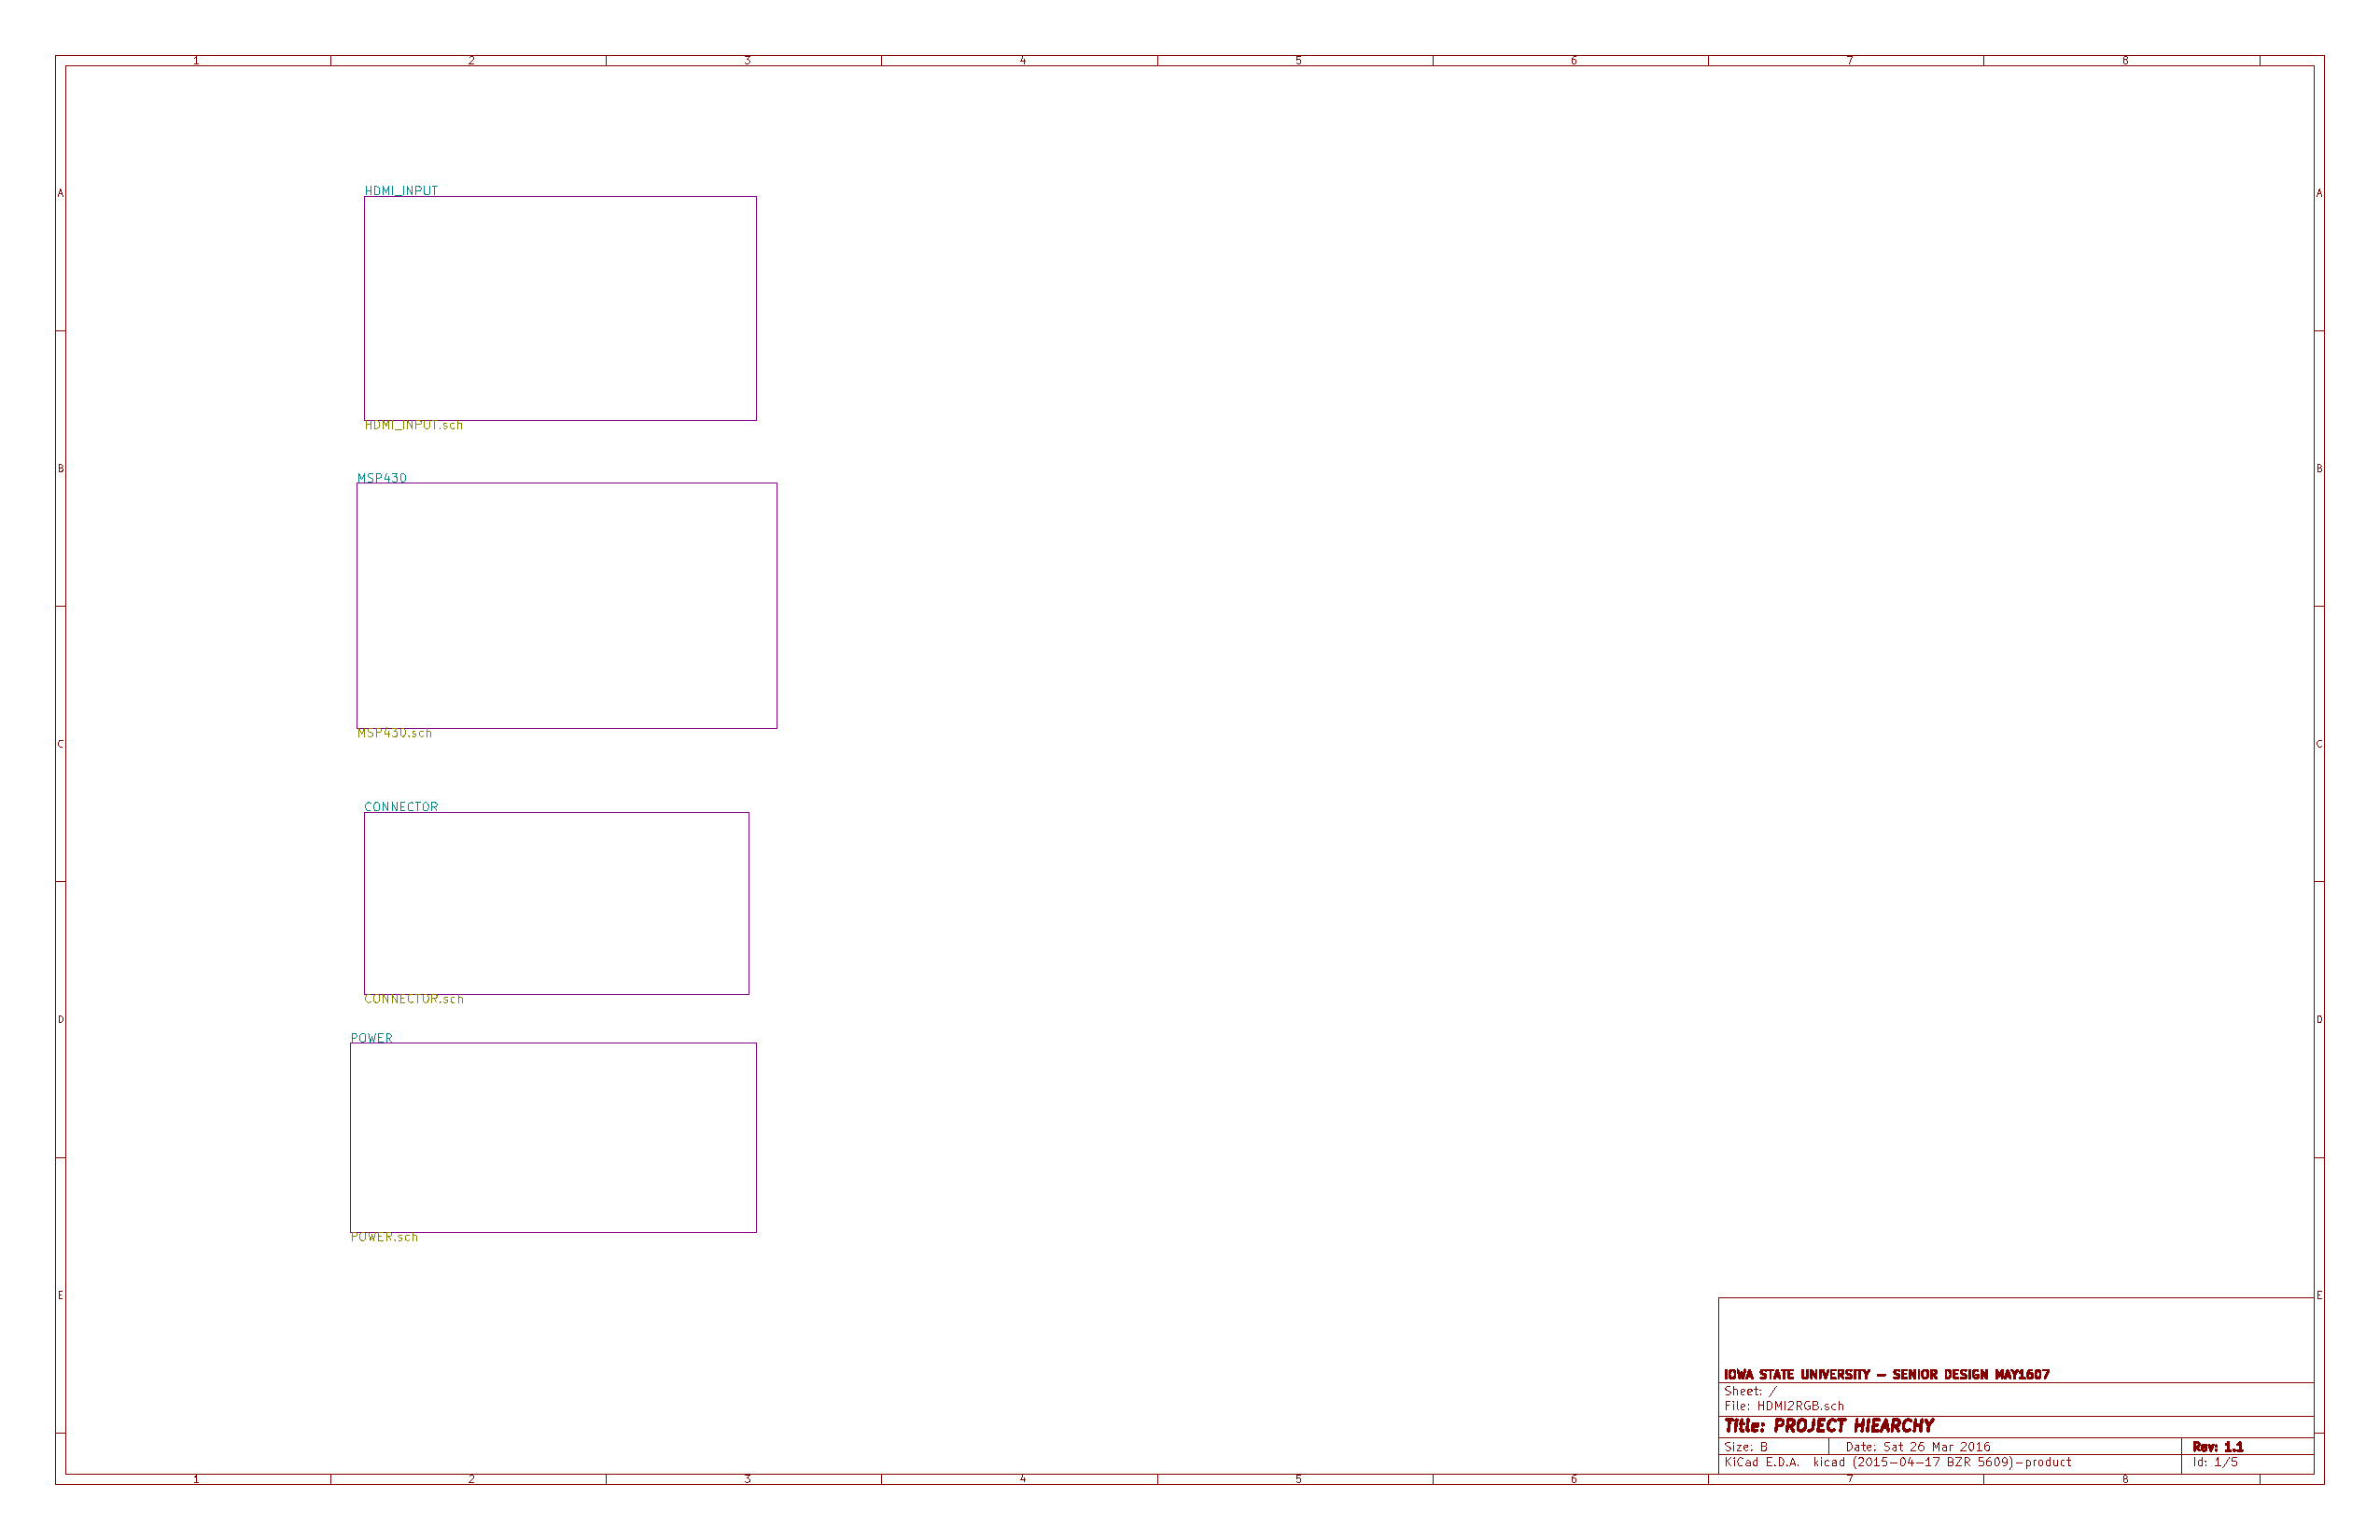
\includepdf[pages=-]{pics/HDMI2RGB.pdf}

\end{appendices}
\end{document}